\clearpage
\twocolumn[
    \section{SAM Units}
]

SAM launcher units are specialized in the destruction of attacking aircraft with surface-to-air missiles.

\subsection{Properties}

Table~\ref{table:infantry-sam-units} summarizes the properties of infantry SAM units, and
Figure~\ref{figure:infantry-sam-units} shows their representation as counters. In addition to the properties shared by all ground units, Table~\ref{table:infantry-sam-units} gives:
\begin{itemize}
    \item the number of ready, volley, and reload missiles;
    \item the multi-target capability;
    \item whether the unit has quick-reaction capability;
    \item whether the unit has IFF capability;
    \item whether the unit has night IR sights; and
    \item the optical lock-on number and range.
\end{itemize}

%the frequency band, range (in mega-hexes) of the EWR, if present, and whether it has a moving-target indicator (MTI) capability; the frequency band and range (in mega-hexes) of the target-tracking radar, if present; the multi-target capability of the unit; the number of ready missiles and the maximum number of missiles in a volley; whether the unit has a quick-reaction capability; its radar and optical lock-on rolls and (for IR SAMs) its lock-on range in hexes.

\subsection{Missile Properties}

Table~\ref{table:sams} summarizes the properties of the actual missiles:
\begin{itemize}
    \item guidance mode;
    \item launch roll;
    \item turn rate;
    \item flight time;
    \item visibility;
    \item ECCM, chaff, and flare ratings;
    \item whether the missile is active homing (AH) or has a home-on-jam (HOJ) capability;
    \item boost phase in FPs;
    \item base speed and sustainer duration in game turns;
    \item minimum altitude (and modifier for targets at T level);
    \item hit rolls for direct and proximity hits; and
    \item damage ratings for direct and proximity hits.
\end{itemize}

%Some missiles have more than one guidance mode (e.g., the SA-2F has an OG backup mode to its CG main mode).

\subsection{Infantry SAM Units}

Infantry SAM units are squads of infantry specialized in the destruction of attacking aircraft with portable SAMs.
Each squad has one launcher and, unless otherwise specified, one ready missile and two reload missiles.

Infantry SAM squads may be attached to infantry, infantry weapons, or infantry HQ platoons.

Most infantry SAMs do not have true proximity fuzes. Thus, proximity hits in the game correspond to glancing direct hits in reality.

\begin{figure}[ht]
    \centering
    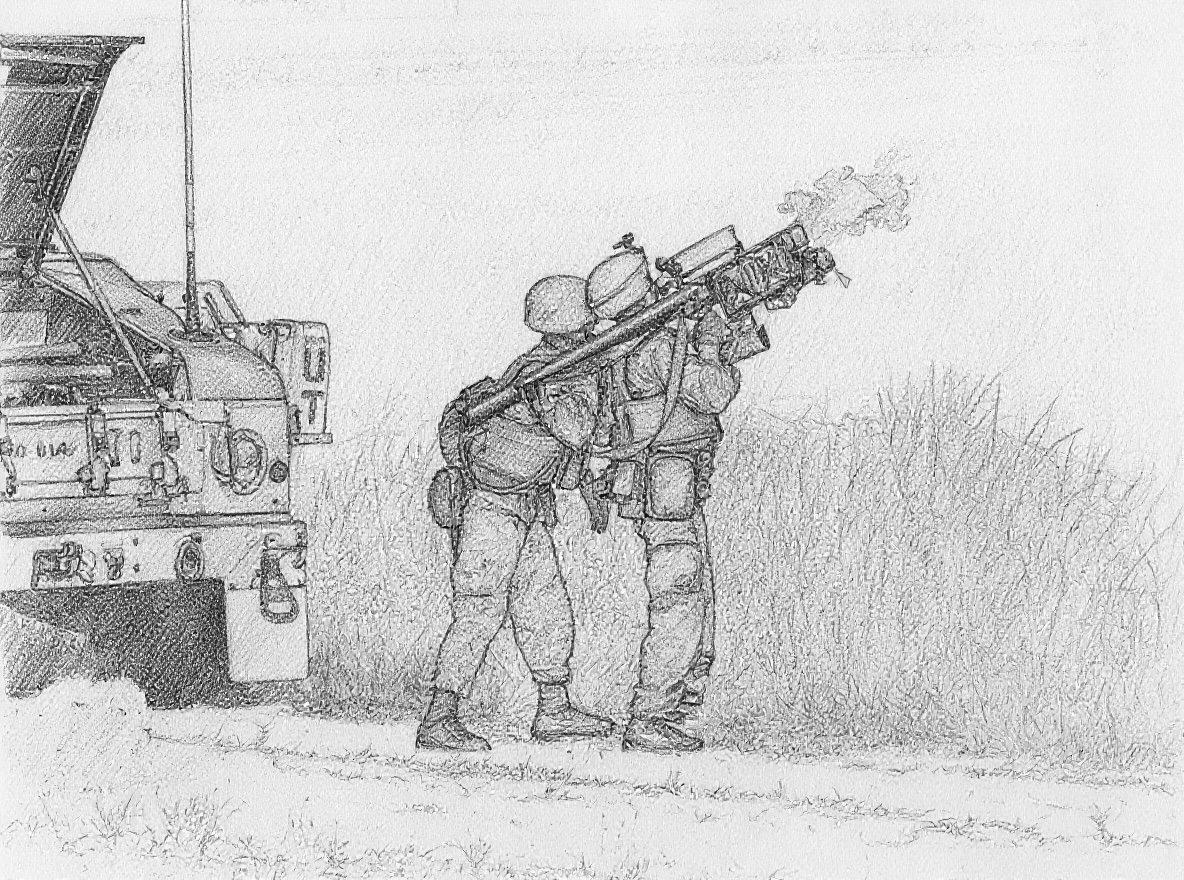
\includegraphics[width=\linewidth]{photos/stinger.jpg}
    % https://commons.wikimedia.org/wiki/File:2nd_LAAD_Marines_fire_an_FIM-92_Stinger.jpg
\end{figure}

\paragraph{SA-7A/B Squad}

The 9K32 Strela-2 (SA-7A Grail) was the first Soviet portable SAM. It has a rear-aspect, uncooled IR seeker.

The 9K32M Strela-2M (SA-7B Grail) is similar, but uses a rear-aspect, electrically-cooled IR seeker.
In Warsaw Pact armies, the Strela-2M was sometimes used with the PRP portable RWR receiver that was capable of passively identifying enemy aircraft by their radar emissions.%
\note{SA-7A Squad}{
    The launcher and SAM values are from \emph{Air Strike} with significant modifications:
    \begin{itemize}
        \item Zaloga gives an in-service date of 1968.
        \item \emph{Air Strike} gives this a seeker type of I, but that does seem appropriate for an uncooled PbS seeker. Instead, I use a seeker type of E, by analogy with the uncooled seeker in the AIM-9B, and works at about 2 microns.
        \item \emph{Air Strike} gives a turn rate of HT, but the control capability seems to be the same as in the SA-7B and SA-15. I will adopt BT.
        \item \emph{Air Strike} gives this a speed of 8. Zaloga gives a lifetime of 8 seconds and an average speed of 1550 km/h. This corresponds to a range of 5.2 km or about 10 hexes.
    \end{itemize}
}%
\note{SA-7B Squad}{
    The launcher and SAM values are from \emph{Air Strike} with significant modifications:
    \begin{itemize}
        \item \emph{Air Strike} gives this a seeker type of I. That seems about right. The seeker was PbS and cooled electrically, like the AIM-9E which also has a type I seeker.
        \item \emph{Air Strike} gives a turn rate of BT, which I adopt.
        \item \emph{Air Strike} gives this a speed of 10. Zaloga states that it has a slightly more powerful rocket motor than the SA-7A, but the mean speed is the same at 1550 km/h. I adopt a speed of 10, like that of the SA-7A.
    \end{itemize}
}

The Strela-2 and -2M entered service with Soviet forces in 1968 and 1970.
They have seen combat in almost every conflict since 1970 in which the Soviet Union or its successor states have been participants or supporters.
In particular, the Strela-2M was used heavily by North Vietnamese forces in the 1973 Easter Offensive, by Arab forces in the 1973 Yom Kippur War, by Angolan forces in the South African Border War, by the Afghan Mujahedeen in the Soviet-Afghan War (having been supplied by the CIA), by Iran in the Iran-Iraq War in the 1980s, and by Serbian and Serbian-supported forces in the Yugoslav Wars in the 1990s.

\paragraph{SA-14 Squad}

The 9K34 Strela-3 (SA-14 Gremlin) is a development of the earlier Strela-2M.
It has a rear-aspect, cryogen-cooled IR seeker.
In Warsaw Pact armies, the Strela-3 was sometimes used with the PRP portable RWR receiver that was capable of passively identifying enemy aircraft by their radar emissions.%
\note{SA-14 Squad}{
    The launcher and SAM values are from \emph{Air Strike} with significant modifications:
    \begin{itemize}
        \item The seeker is cryogenically cooled at works at about 4 microns (Zaloga). \emph{Air Strike} gives this a type A seeker, but that does seem appropriate; the first type A seekers in Soviet AAMs did not appear until 1985 in the AA-8C. Also, type A seekers have all-aspect capability Zaloga says that the seeker has similar performance to the RIM-43C, but only limited all-aspect capability. A type M seeker seems to be more appropriate.
        \item \emph{Air Strike} gives a turn rate of ET, but the control capability seems to be the same as in the SA-7A and SA-7B. I will adopt BT.
        \item \emph{Air Strike} gives this a speed of 12. Zaloga gives a lifetime of 8 seconds and an average speed of 1440 km/h (as it is slightly heavier than the SA-7). This corresponds to a range of 4.8 km or about 9 hexes.
        \item The warhead is the same as on the SA-7A/7B.
    \end{itemize}
}

The Strela-3 entered service with the Soviet Army in 1974.
It has seen combat in many conflicts since then in which the Soviet Union or its successor states have been participants or supporters.
In particular, it was used by Iraqi forces in the 1991 Gulf War.

\paragraph{SA-16/18 Squad}

9K310 Igla-1 (SA-16 Gimlet) and 9K38 Igla (SA-18 Grouse) use very similar missiles and launchers, but the Igla-1 has a single-channel IR seeker similar to the SA-14, and the Igla uses a dual-channel IR seeker to reduce its susceptibility to flares.
The warhead was similar to the SA-7/14, but also exploded any remaining rocket fuel.
In the game, this is simulated by increasing the damage rating by one if the missile attacks before expending more than half of its FPs (round down).
Both incorporate IFF interrogators, but these were only used in Warsaw Pact armies.%
\note{SA-16/18 Squad}{
    The launcher and SAM values are from Malcolm Pipes with significant modifications:
    \begin{itemize}
        \item The warhead of the SA-16/18 is 1.17 kg, identical to the 1.17 kg of the SA-7 and similar to the 1.1 kg of the SA-14. Only later Iglas had heavier warheads. Therefore, I have reduced the damage ratings to match the SA-7.
        \item Carl comments that the warhead explodes any remaining rocket fuel. I increase the damage rating by one if the target is reached in the first half of the FPs.
        \item I have reduced the lock-on range of the SA-16 to match that of the SA-14.
        \item I have increased the flare rating of the SA-16 to match that of the SA-14.
        \item I have given both missiles the same speed and turn rate. Zaloga states that the engagement range increased by about 1 km with respect to the SA-7/14, so I am increasing the speed by 2 to 12. I will give both a turn rate of BT/2, matching Stinger.
    \end{itemize}
}

The Igla-1 entered service with the Soviet Army in 1981 and the Igla in 1983.
Both have been widely exported and have seen combat in many conflicts since then in which the Soviet Union or its successor states have been participants or supporters.
The Igla was used by Iraqi forces in the 1991 Gulf War, by the Peruvian Army in the 1995 Cenepa War, and by Serbian forces in the 1999 Kosovo War.

\paragraph{FIM-43C Squad}

The FIM-43C Redeye Block III was the first US infantry SAM to reach production and enter service.
It has a rear-aspect, cryogen-cooled IR seeker.%
\note{FIM-43C Squad}{
    The launcher and SAM values are from \emph{Air Strike}.
}

The FIM-43C entered service with the US Army in 1968 and subsequently was used by Australia, Chad, Denmark, West Germany, Greece, Israel, Jordan, Saudi Arabia, Somalia, Sudan, Sweden, and Turkey. It was also supplied by the CIA to the Afghan Mujahedeen and the Nicaraguan Contras.

\paragraph{FIM-92A/B/C/D Squad}

The FIM-92A Stinger has an all-angle, second-generation, cryogen-cooled IR seeker.
Its warhead weight 3 kg and was significantly more lethal than in earlier missiles.
The FIM-92B Stinger POST adds a UV seeker to distinguish flares from aircraft.
The FIM-92C/D Stinger RMP have software updates to further improve the performance against flares.
All have an IFF interrogator to help avoid fratricide.%
\note{FIM-92A/B/C/D Squad}{
    The launcher and SAM values for the A model are from \emph{Air Strike}. Those for the B/C/D models are from Malcolm Pipes compendium.
    \begin{itemize}
        \item I have increased the flare susceptibility of the FIM-92A from 2 to 3. It did not seem to have significant protection.
        \item Wikipedia gives an effective range of 5 miles, which is equivalent to a speed of 15. I have left the speed at 14, as that is close enough.
        \item Wikipedia gives a peak speed of 1930 mp and a self-destruct time of 17 seconds.
        \item \emph{Air Strike} has the visibility as 2, but looking at photos I don't see much differ
    \end{itemize}
}

The FIM-92A entered service with the US Army in 1981, the FIM-92B in 1986, the FIM-92C in 1989, and the FIM-92D in 1992. They were exported to dozens of US allies including the Afghan Mujahedeen and the Angolan UNITA. They saw service in the 1982 South Atlantic War, the Soviet-Afghan War, the Angolan Civil War, the Libyan Invasion of Chad, the Tajik Civil War, the Chechen War, the Sri Lankan Civil War, the Syrian Civil War, and the Russian Invasion of Ukraine.

\paragraph{Blowpipe Squad}

Blowpipe is an MCLOS optically-guided missile.
While in theory this gave it an all-aspect capability, in practice guiding the missile to the target in combat proved to be very difficult.%
\note{Blowpipe Squad}{
    The launcher and SAM values are from \emph{Air Strike}.
}

Blowpipe entered service with the British Army and Royal Marines in 1975.
It was also used by the Argentine Army, Canadian Army, Chilean Army and Navy, Ecuadorean Army, Guatemalan Army, Portuguese Army, Malawian Army, Malaysian Army, Nigerian Army, Omani Army, Royal Thai Air Force and Army, and the UAE Army.
It saw combat in the 1982 South Atlantic War with both sides and had a low success rate.
In 1986, it was trialed by the Afghan Mujahedeen, but again was not considered to be effective.
Finally, it was also used in the 1995 Cenepa War by Ecuador.

\paragraph{Javelin/Starburst Squad}

Given the poor performance of Blowpipe in the 1982 South Atlantic War, Javelin was quickly developed as an upgraded version of Blowpipe with SACLOS guidance in place of MCLOS guidance. Starburst then replaced the radio-link with laser guidance. Javelin is also called “Javelin GL” and Starburst was originally called “Javelin S15”.%
\note{Javelin/Starburst Squad}{
    The launcher and SAM values for Javelin are from \emph{Air Strike}. The launcher and SAM values for Javelin are just those for Javelin but with the OG guidance replaced by LG guidance. I have seen mention of a Javelin LML; did anyone use it or was it just a prototype?
}

Javelin replaced Blowpipe in the British Army and Royal Marines in 1984.
It was also used by the Botswana Army, the Canadian Army, the Malaysian Army, the Peruvian Army, and the South Korean Army.

Starburst in turn replaced Javelin in the British Army and Royal Marines in 1989.
It was also used by the Canadian Army, the Malaysian Army, the Qatari Army, and the Royal Thai Army.
Starburst served with the British Army in the 1991 Gulf War, but was not used in combat.

\paragraph{Starstreak Squad}

Starstreak is a high-speed laser-guided missile. As the missile approaches the target, it launches three independent explosive darts. The darts have contact fuzes, but not proximity fuzes.%
\note{Starstreak Squad}{
    The launcher and SAM values are from Malcolm Pipes. The real darks do not have proximity fuzes, but the missile in the game can obtain a proximity hit. Perhaps a proximity hit here means a hit with only one die?
}

Starstreak replaced Javelin in the British Army and Royal Marines in 2000 and is also used by the South African Army and the Armed Forces of Ukraine.
Starstreak served with the British Army in the 2003 Invasion of Iraq, but was not used in combat. It has seen combat in the Russian Invasion of Ukraine.

\paragraph{Starstreak LML Squad}

The Starstreak Light Multiple Launcher (LML) has three ready-to-fire Starstreak missiles on a pedestal mount with a single sighting unit. The launcher and its associated equipment are heavy and will normally be transported by a vehicle unit.%
\note{Starstreak LML Squad}{
    The SAM values are from Malcolm Pipes. I have guessed the launcher values are the same as for shoulder-launched version, just that the launcher has three ready missiles. I don't know if the launcher has reloads. Is the launcher really portable or does it have to be transported by a vehicle?
}

Starstreak LML entered service with the British Army and Royal Marines in 2000.
It is also used by Indonesia, Malaysia, and South Africa.

\paragraph{Mistral Squad}

The Mistral is a French IR-homing missile on a pedestal mount. The missile has a considerably larger warhead than either the Stinger or Igla missiles, but this comes at a cost in portability. The launcher and its associated equipment are heavy and will normally be transported by a vehicle unit.%
\note{Mistral Squad}{
    The launcher and SAM values are from \emph{Air Strike}. Is the launcher really portable or does it have to be transported by a vehicle?
}

The Mistral entered service with the French Army in 1990. It was subsequently exported to many other countries.

\paragraph{RBS 70 Squad}

The RBS 70 is a Swedish laser-guided missile on a pedestal mount. The launcher and its associated equipment are heavy and will normally be transported by a vehicle unit.%
\note{RBS 70 Squad}{
    For the RBS 70: The launcher and SAM values are from \emph{Air Strike}. Is the launcher really portable or does it have to be transported by a vehicle?
}

The RBS 70 entered service with the Swedish Army in 1977. It was subsequently used by Argentina, Australia, Bahrain, Brazil, the Czech Republic, Iran, Ireland, Lithuania, Norway, Pakistan, Singapore, Thailand, Tunisia, the UAE, Ukraine, and Venezuela.

\paragraph{Ayn-al-Saqr Squad}

The Ayn-al-Saqr (“Eye of the Hawk”) missile is a  licensed version of the 9M32M Strela-2m (SA-7B Grail) manufactured in Egypt. It equips one version of the Sinai 23 air-defense vehicle.%
\note{Ayn-al-Saqr Squad}{
    The launcher and SAM values are taken to be equal to those of the SA-7B.
}

It entered service with the Egyptian Army in 1984.

\subsection{Vehicular and Towed SAM Units}

\begin{figure*}
    \centering
    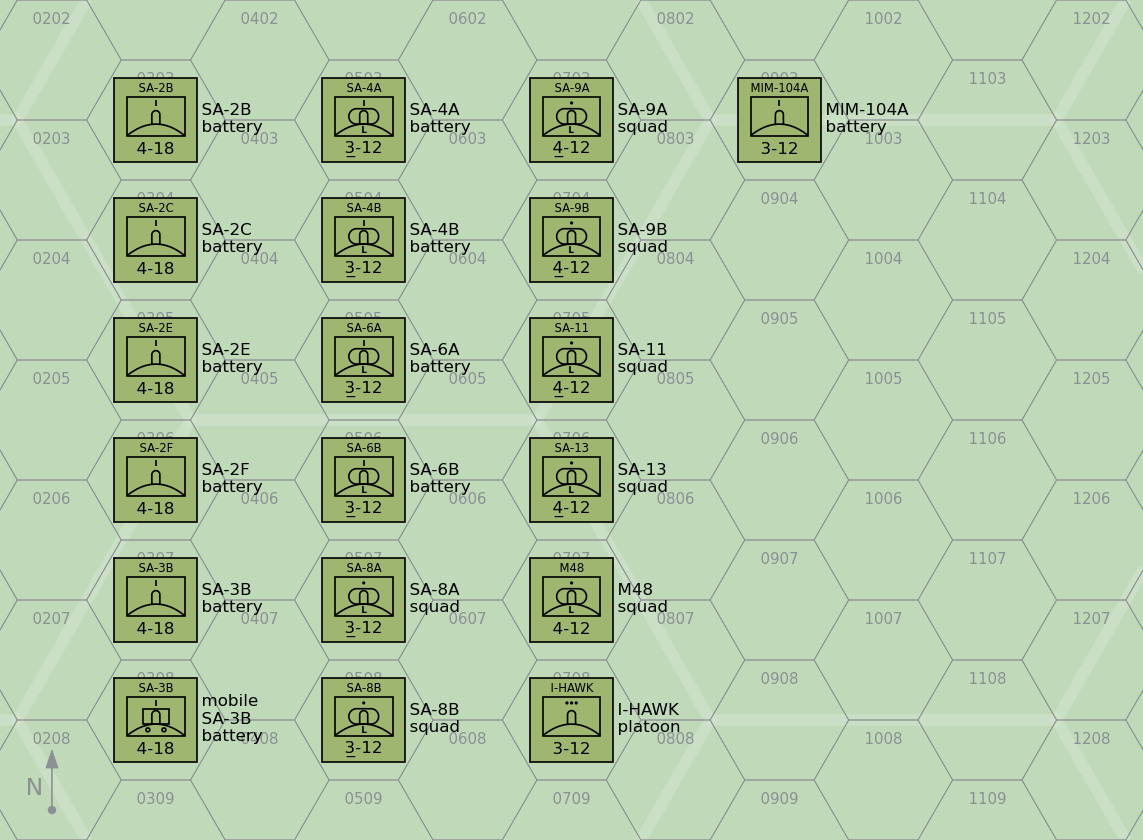
\includegraphics[width=0.8\linewidth]{figure-sam-launcher.png}
    \caption{SAM Launcher Units}
    \label{figure:sam-launcher-units}
\end{figure*}

\paragraph{Echelon}
The size of a SAM launcher unit is squad, section, or platoon according to its damage resilience (1D, 2D, or 3D, respectively).
This does not always coincide with the actual designations used historically. For example, the SA-2 battery in the game corresponds to a battalion in reality.

\paragraph{Nuclear Warheads}
The SA-2E has the option of a nuclear warhead.

\subsection{Soviet and Russian SAM Launcher Units}

\paragraph{SA-2B/C/E/F Battery}

This is an S-75 (SA-2 Guideline) battery of six single launchers for the long-range V-750 missile and their associated P-12 (Spoon Rest) EWR and SNR-75 (Fan Song) TTR. The variants are the S-75 Desna (SA-2B), S-75M Volkhov (SA-2C), S-75AK (SA-2E), and S-75SM (SA-2F).
All are radar-guided, but the SA-2F also has an optical backup.

The S-75 Dvina (SA-2A) system was deployed by the Soviet PVO in 1957. In addition to serving as a key part of the air-defense system of the Soviet Union (and its notable role in ending reconnaissance overflights by shooting down the U-2 of Gary Powers) and its allies, it saw combat in Cuba in 1962, with North Vietnamese forces from 1965, with Indian forces in the 1965 war with Pakistan, and with Egyptian and Syrian forces from 1967.

\paragraph{SA-3B Battery}

This is an S-125 Neva (SA-3B Goa) battery with four quad launchers for the 5V24 missile and their associated P-15 (Flat Face) EWR and SNR-125 (Low Blow) TTR.

It saw combat with Egyptian and Syrian forces from 1970.

\paragraph{Mobile SA-3B Battery}

This is a mobile S-125 Neva (SA-3B Goa) battery with four twin launchers for the 5V24 missile on trucks and their associated P-15 (Flat Face) EWR and SNR-125 (Low Blow) TTR.

It saw combat with Egyptian and Syrian forces from 1970 and with Iraqi forces in the Iran-Iraq War, the Gulf War, and the Invasion of Iraq.

\paragraph{SA-4A/B Battery}

This is an armored 2K11 Krug (SA-4A/B Ganef) battery with three launcher vehicles each with two long-range 9M8M1/9M8M2 missiles and their associated P-40 (Long Track) EWR and 1S32 (Pat Hand) TTR.

It saw combat with Egyptian and Syrian forces from 1970 and with Iraqi forces in the Iran-Iraq War, the Gulf War, and the Invasion of Iraq.

\paragraph{SA-6A/B Battery}

This is an armored 2K12 Kub (SA-6A/B Gainful) battery with four launcher vehicles, each with three medium-range 2K12 Kub (SA-6A) or 3M9M3 (SA-6B) missiles and their associated P-40 (Long Track) EWR and 1S32 (Pat Hand) TTR.

It saw combat with Egyptian and Syrian forces from 1970 and with Iraqi forces in the Iran-Iraq War, the Gulf War, and the Invasion of Iraq.

\paragraph{SA-8A/B Squad}

This is a squad with a single 9K33 Osa or 9K33M Osa-AK (SA-8A/B Gecko) vehicle with integrated 1S51M3 (Land Roll) TTR.
The SA-8A carries four 9M33 missiles, and the SA-8B carries six 9M33M missiles.

The Osa has been widely exported and seen combat with Syrian forces in the 1982 Lebanon War, with Cuban forces in the South African Border War, with Iraqi forces in the 1990 Gulf War, and in more recent conflicts.

\paragraph{SA-9A/B Squad}

This is a squad with a single 9K21 Strela-1 or 9K21M Strela-1M (SA-9A/B Gaskin) vehicle with four 9M21 or 9M21M missiles.
In the Soviet army, a platoon of four was assigned to the air-defense battery of tank and motor-rifle regiments, complementing the ZSU-23-4.

The Strela-1 has been widely exported and saw combat in the South African Border War, the Iran-Iraq War, the Lebanon War, the Gulf War, the Kosovo War, and the Invasion of Iraq.

\paragraph{SA-11 Squad}

This is a squad with a single 9K37 Buk (SA-11 Gadfly) vehicle with four 9M37 missiles and an integrated 9S35 (Fire Dome) TTR. Three squads make up a battery, and three batteries make up a battalion. Normally, one armored 9S18 (Tube Arm) or 9S18M1 (Snow Drift) EWR is allocated to each battalion.

The SA-11 has seen combat in the War in Abkhazia, the Russo-Ukrainian War, and during the Syrian Civil War.

\paragraph{SA-13 Squad}

This is a single 9K35 Strela-10 (SA-13 Gopher) vehicle with four infra-red homing 9M37 missiles. Four squads form a platoon.
It began to replace the SA-9B in the air-defense platoons of tank and motor-rifle regiments in the Soviet Army starting in 1976 and was subsequently widely exported to Soviet allies.
Compared to the earlier system, the missile offers greater lethality, and the vehicle greater protection and mobility (although it is not amphibious).
Some are equipped with 9S16 (Flat Box-B) RWR.

The SA-13 saw combat in the South African Border War with Angolan forces, the Gulf War with Iraqi forces, and in the Kosovo War with Serbian forces.

\subsection{US SAM Launcher Units}

\paragraph{M48 Squad}

This is a single M48 Chaparral vehicle with four adapted Sidewinder infrared-homing missiles. It was developed after the ambitious Mauler SAM program was abandoned and introduced in 1969. Night IR sights were added in 1984 to give it a limited night capability. The MIM-72A was the original missile based on the AIM-9D. The MIM-72C added an improved seeker and warhead, and the MIM-72E/F added a smokeless motor. The final MIM-72G added a seeker based on that of the FIM-92B Stinger, with much improved rejection of infrared countermeasures.

\paragraph{I-HAWK Platoon}

This consists of three triple launchers for the MIM-23A/C/D missile, plus supporting radars and command elements.
The MIM-23B Improved HAWK and its associated improved radars were developed from the original HAWK MIM-23A to give much improved performance at low levels.
The MIM-23C has improved ECCM, and the MIM-23D adds a home-on-jam capability.
Two platoons with an EWR make up a battery.

The I-HAWK was deployed by the US Army, US Marines, and many US allies.

\paragraph{MIM-104 Battery}

An MIM-104 Patriot battery consists of six launchers with associated radar and command elements.
The MIM-104A uses the “Standard” missile and was capable only of defense against aircraft.
Patriot is used by the US Army and numerous US allies.

\begin{figure*}[p]
    \centering
    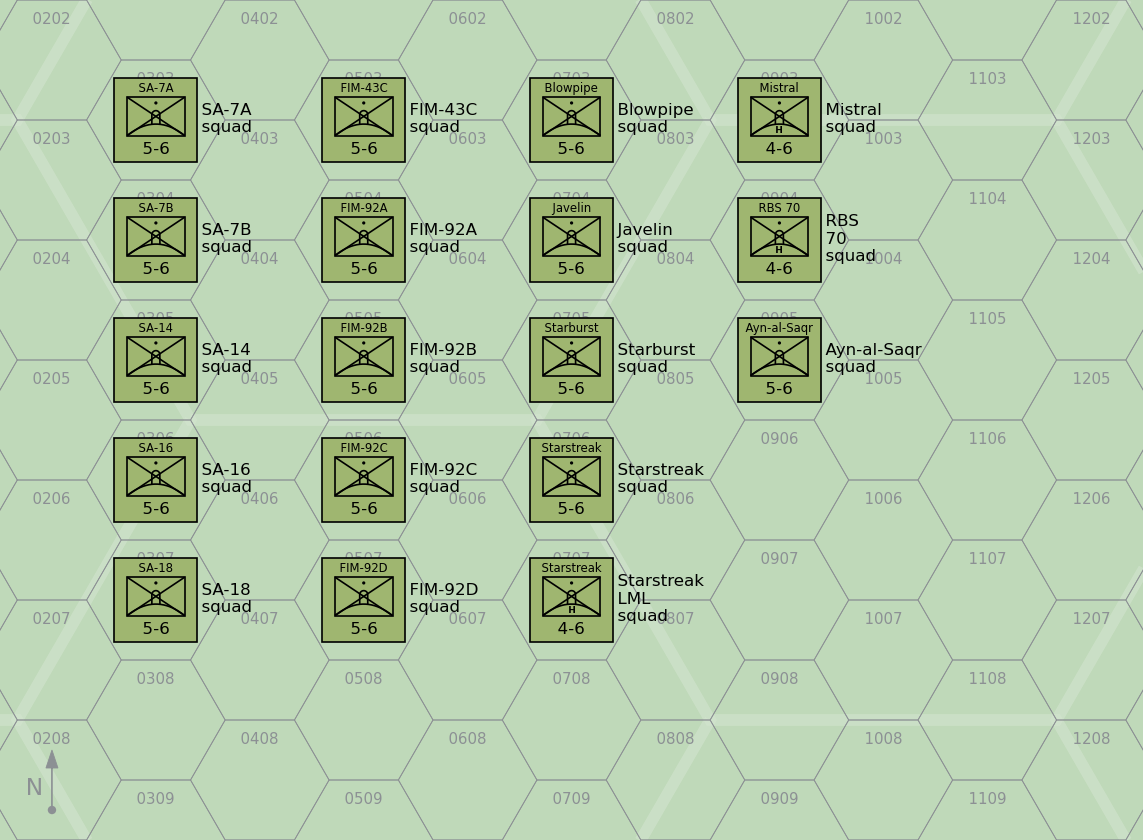
\includegraphics[width=0.8\linewidth]{figure-infantry-sam-units.png}
    \caption{Air-Defense Units: Infantry SAM Units}
    \label{figure:infantry-sam-units}
\end{figure*}

\begin{table*}[p]
    \caption{Air-Defense Units: Infantry SAM Units}
    \centering
    \footnotesize
    \input{table-infantry-sam-units.tex}
    \label{table:infantry-sam-units}
\end{table*}

\begin{table*}[p]
    \caption{Air-Defense Units: SAM Launcher Units}
    \centering
    \footnotesize
    \input{table-sam-launcher-units.tex}
    \label{table:sam-launcher-units}
\end{table*}

\begin{table*}[p]
    \caption{SAMs}
    \centering
    \footnotesize
    \input{table-sams.tex}
    \label{table:sams}
\end{table*}
